See 
\figref{fig:chapters/10/7/3/4/Fig1}
\begin{figure}[H]
 \begin{center}
  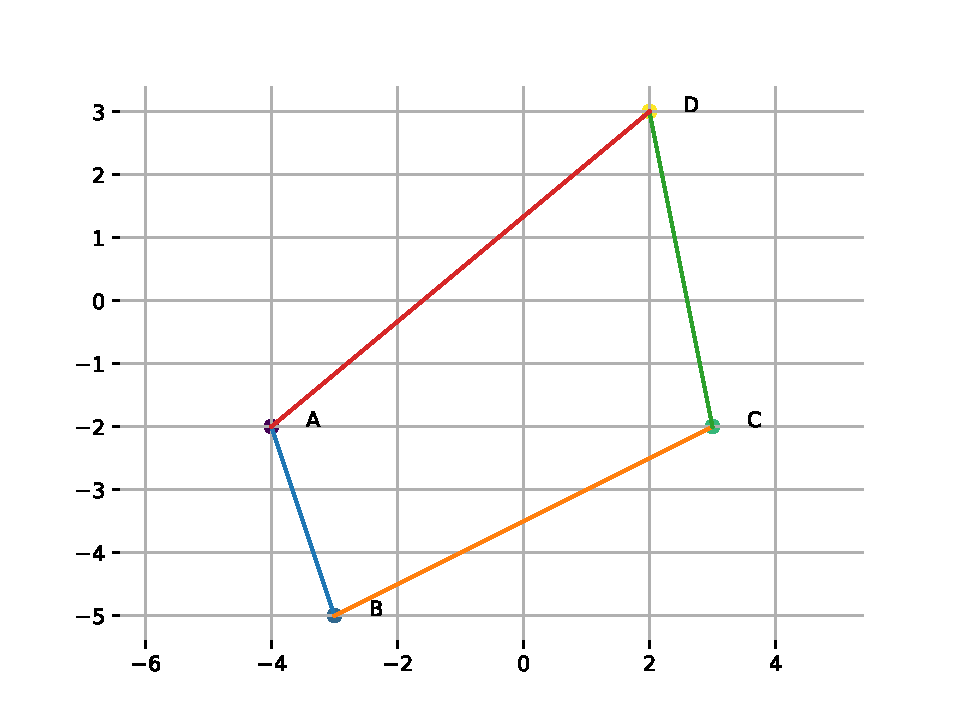
\includegraphics[width=0.75\columnwidth]{chapters/10/7/3/4/figs/fig.pdf}
 \end{center}
\caption{}
\label{fig:chapters/10/7/3/4/Fig1}
\end{figure}
\begin{align}
\because	\vec{A}- \vec{B} =\myvec{-1\\3},\,
	  \vec{A}- \vec{D} =\myvec{-6\\-5},
	  \\
	\vec{B}- \vec{C} =\myvec{-6\\-5},\,
	  \vec{B}- \vec{D} =\myvec{-3\\-8},
	  \\
	  ar(ABD)=\frac{1}{2} \norm{\brak{\vec{A}-\vec{B}}  \times 
   \brak{\vec{A}- \vec{D}}} 
	=	\frac{23}{2}
	\\
	  ar(BCD)=\frac{1}{2} \norm{\brak{\vec{B}-\vec{C}}  \times 
   \brak{\vec{B}- \vec{D}}} 
	=	\frac{33}{2}
	\\
\implies	ar(ABCD)=  ar(ABD) +  ar(BCD)
	= 28
\end{align}
